\documentclass{llncs}
\usepackage{amssymb}
\usepackage{graphicx}
\usepackage[ruled,linesnumbered,boxed]{algorithm2e}
\usepackage{graphicx}
\usepackage{amsmath}
%\usepackage{mathtools}
%\usepackage{color}
\usepackage{tabularx}
\usepackage[colorlinks, linkcolor=blue, anchorcolor=blue, citecolor=green]{hyperref}
%\usepackage{booktabs}
\usepackage[table]{xcolor}
%\uespackage{colortbl}
\usepackage[tight,footnotesize]{subfigure}
\usepackage{fancyhdr}
\usepackage{lastpage}
\usepackage{layout}
\usepackage{appendix}
\usepackage{ctex}
\usepackage{float}
\usepackage{multirow}
\usepackage{booktabs}
\usepackage{comment}
\usepackage{listings}

\usepackage{indentfirst}
\setlength{\parindent}{2em}

\lstset{
	flexiblecolumns,                                     % 别问为什么,加上这个
	numbers=left,                                        % 在左侧显示行号
	breaklines=true,   									 % 自动换行,建议不要写太长的行
	numberstyle=\tiny\color{gray},                       % 设定行号格式
	frame=none,                                          % 不显示背景边框
	backgroundcolor=\color[RGB]{245,245,244},            % 设定背景颜色
	keywordstyle=\color[RGB]{40,40,255},                 % 设定关键字颜色
	numberstyle=\footnotesize\color{darkgray},           
	commentstyle=\it\color[RGB]{0,96,96},                % 设置代码注释的格式
	stringstyle=\rmfamily\slshape\color[RGB]{128,0,0},   % 设置字符串格式
	showstringspaces=false,                              % 不显示字符串中的空格
	language=c++,                                        % 设置语言
}

%\footskip = 10pt
\pagestyle{fancy}
\chead{Group Project}
\lhead{CS2308-Algorithm@SJTU}
\rhead{Instructor: Xiaofeng Gao}
\rfoot{}
\cfoot{Page \thepage \ of \pageref{LastPage}}
\addtolength{\headheight}{0.5\baselineskip}
\addtolength{\headwidth}{0\marginparsep}
\addtolength{\headwidth}{0\marginparwidth}



\title{SACG: Simulated Annealing Combined with Greedy Algorithm}
\subtitle{An Approximation Solution to \\ Resource Scheduling Problem in Hadoop}

\author{Zhenran Xiao, Zichun Ye, Mabiao Long \\
	Student ID:\{520030910281, 520030910302, 520030910308\} \\
	\{xiaozhenran, alchemist, albertlong007\} @ sjtu.edu.cn
}
\institute{Department of Computer Science and Engineering, \\ Shanghai Jiao Tong University, Shanghai, China}

\begin{document}
	\bibliographystyle{plain}
	
	%\linespread{0.85}
	
	%==============================================================================
	\maketitle
	\begin{abstract}\vspace{-5mm}
		
		The course project focuses on resource scheduling problem in Hadoop. This document first introduce the background and two versions of resource scheduling on single or multiple hosts. Then it designs an algorithm based on simulated annealing algorithm and greedy algorithm to give an approximate solution to the problems of two versions. It also does some experiments on parameters in the algorithm and analyses the complexity and other quality of the algorithm.  
		
		\textbf{Keywords:} Distributed Computing System, Resource Scheduling, Hadoop, Simulated Annealing Algorithm, Greedy Algorithm, NP-complete problem
	\end{abstract}
	
	\section{Background and Motivation}
	\label{sec-Hadoop}
	
	Hadoop is an open-source software framework for storing data and running applications on clusters of commodity hardware. In Hadoop, the data of a running job can be divided into several data blocks, stored on different hosts. Each host has one or multiple CPU cores to process data blocks. In this project, our goal is to achieve effective parallel computing. That is to say, given a set of jobs with massive data, we need to design a resource scheduling algorithm to minimize the overall executing time of all jobs.
	
	
	
	\section{Problem Formulation and Explanation}
	\label{sec-problem}
	In this section, we will formulate the problem and explain some definitions.
	
	\subsection{A Simplified Version with Single Host} \label{subsec-task1}
	
	First, let us consider a simple case with a single host storing all data blocks. To simplify the problem, we give the following assumptions and specifications.
	
	\begin{enumerate}
		
		\item There are $n$ jobs that need to be processed by a single host, which has $m$ CPU cores of the same computing capability. Let $J$ be the set of jobs, and $C$ be the set of cores for the host, where $J = \{job_0, job_1, \cdots, job_{n-1}\}$, and $C = \{c_0, c_1, \cdots, c_{m-1}\}$ (The labels of variables start from 0 because we use C/C++ source codes in the following tasks).
		
		\vspace{2mm} 
		
		\item We treat data block as the smallest indivisible unit in our project, while a job can be divided into multiple data blocks with different sizes for storage and computing. Assume $job_i$ is split into $n_i$ data blocks, denoted by $B^i = \{b^i_{0}, b^i_{1}, \cdots, b^i_{n_i-1}\}$. For block $b^i_{k}$ of $job_i$, define its size as $size(b^i_{k})$.
		
		\vspace{2mm} 
		
		\item Assume $job_i$ is assigned to $e_i$ cores for processing, and naturally $e_i \leq n_i$. That is to say, one core can process multiple data blocks of one job sequentially. Let $B^i_{j}\subseteq B^i$ denote the set of data blocks of $job_i$ allocated to core $c_j$, and $B^i_{j} \cap B^i_{j'} = \varnothing$ if $j \neq j'$ (they should be disjointed). 
		
		\vspace{2mm} 
		
		\item For $job_i$, the processing speed of its data blocks is $s_i$ when $job_i$ is assigned to a single core. However, when multiple cores process $job_i$ in parallel, the computing speed of each core all decays because of some complicated interactions. We formulate such speed decay effect caused by multi-core computation as a coefficient function $g(\cdot)$ with respect to core number $e_i$, as described in Equation~\eqref{Eq-decay}:
		\begin{equation} \label{Eq-decay}
			g (e_i) = 1.00 - \alpha \cdot (e_i-1), \quad  \text{for} \ 1 \leq e_i \leq 10,
		\end{equation}
		where $\alpha$ is a decay factor satisfying $0 < \alpha < 1$ , and usually the number of cores for processing a single job is no more than 10. Then, the speed of each core can be rewritten as $s_i \cdot g(e_i)$ for $job_i$ respectively. (Note that although the speed of each core decays, the overall processing time using $e_i$ cores in parallel should be faster than that of using just one core. Otherwise we do not need to implement parallel computing. Thus the setting of $\alpha$ should guarantee this principle.)
		
		\qquad Correspondingly, the processing time $tp^i_{j}$ of core $c_j$ for $job_i$ can be expressed as Equation~\eqref{Eq-process}:
		\begin{equation} \label{Eq-process}
			tp^i_{j} = \frac{\sum_{b^i_{k} \in B^i_{j}}size(b^i_{k})}{s_i \cdot g(e_i)}.
		\end{equation} 
		
		\vspace{2mm}
		
		\item For consistency issues, if we assign a job to multiple cores, all cores must start processing data blocks at the same time. If one or several cores are occupied by other affairs, then all other cores should wait for a synchronous start, and keep idle. It means that the processing of $job_i$ for every core should all start at time $t_i$, whereas their processing duration might be different. Let $tf^i_{j}$ be the finishing time of core $c_j$ for $job_i$, which is calculated by Equation~\eqref{Eq-finish}:
		\begin{equation} \label{Eq-finish}
			tf^i_{j} = t_i + tp^i_{j}.
		\end{equation}   
		
		However, the occupied cores of $job_i$ are released synchronously when the computing process of the last data block is finished. Thus the finishing time $tf(job_i)$ of $job_i$ is given as Equation~\eqref{Eq-jobfinish}:
		\begin{equation} \label{Eq-jobfinish}
			tf(job_i) = \max_{c_j} \; tf^i_{j}, \text{ for } c_j \in C.
		\end{equation} 
	\end{enumerate}
	
	\subsection{A Comprehensive Version among Multiple Hosts} \label{subsec-task2}
	
	In this section, we consider a more complex situation, where we need to schedule resources among multiple hosts. Now the data transmission process between pairwise hosts should be taken into consideration. The data blocks of jobs could be initially stored on different hosts, but one data block can only be initially stored on one specified host. If data block $b^i_{k}$ and its assigned computing core $c_j$ are not on the same host, $b^i_{k}$ will be transmitted to the host containing $c_j$ (Here we assume that the bandwidth between hosts is sufficient for data transmission). The transmission process will influence the finishing time of jobs, further affecting the resource scheduling process.
	
	Besides the descriptions and specifications of Section~\ref{subsec-task1}, here are more notations and explanations.
	
	\begin{enumerate}
		
		\item Assume we have $q$ hosts $H=\{h_0, h_1, \cdots, h_{q-1}\}$, and host $h_l$ has $m_l$ cores (may have different number of cores). Let $C_l$ be the set of cores on host $h_l$, $C_l = \{c^l_0, c^l_1, \cdots, c^l_{m_l-1}\}$. Easy to see, $\sum_{l=0}^{q-1} m_l = m$.
		
		\vspace{2mm}
		
		\item If core $c^l_j$ on host $h_l$ computes a data block $b^i_{k}$ of $job_i$ which is initially stored on another host $h_l'$, then $b^i_{k}$ needs to be transmitted from $h_l'$ to $h_l$ at a transmission speed $s_t$ (this speed is fixed in our system). An example is shown in Figure~\ref{Fig-Transmission}, where hosts $h_0$ and $h_1$ both have two cores, and many jobs need to be processed. Core $c^1_0$ on host $h_1$ is assigned to compute the data block $b^1_2$ of $job_1$, which is initially stored on host $h_0$. In this case, $b^1_2$ needs to be transmitted from $h_0$ to $h_1$ at a transmission speed $s_t$ first, and then be computed by $c^1_0$. Whenever $b^1_2$ starts transmission, other cores can work in parallel to process $job_1$.
		
		\begin{figure}[H]
			\begin{center}
				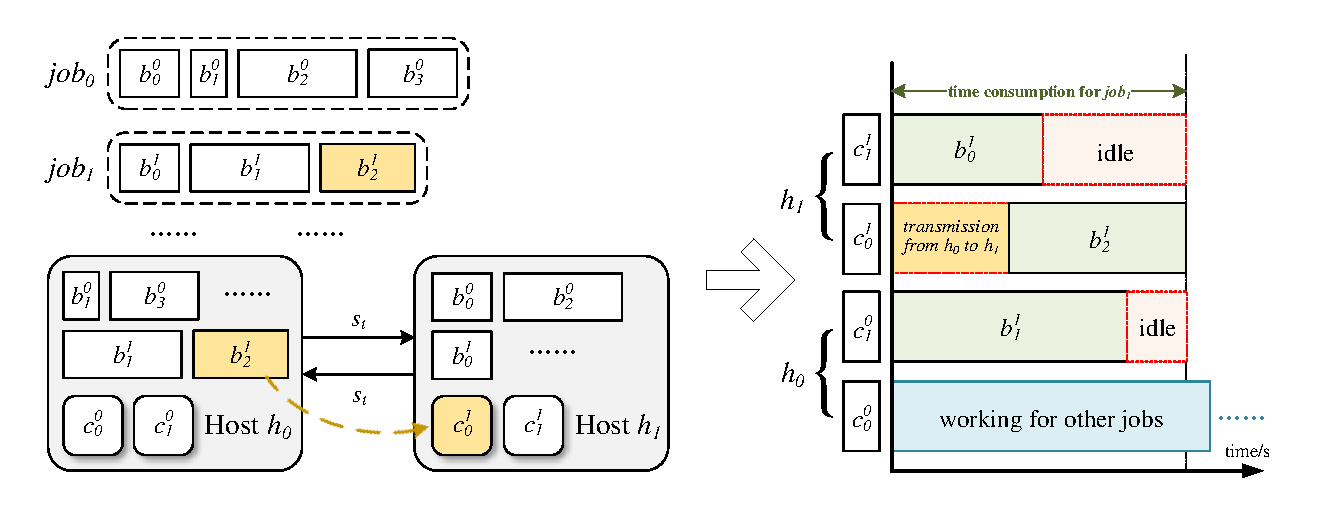
\includegraphics[width=0.9\textwidth]{Fig-Transmission.pdf}
				\caption{An example of data transmission between 2 hosts}
				\label{Fig-Transmission}
			\end{center}
		\end{figure}
		
		\item Any core cannot call for data transmission when it is calculating other data blocks. Likewise, a core cannot start computing any data block until this block is ready, i.e. initially on the same host or transmitted from a remote host to the local host. For example, the core $c^1_0$ on host $h_1$ must wait for the data transmission of block $b^1_2$ from host $h_0$ to $h_1$, and then start computation. What is more, the transmission time of $b^1_2$ from $h_0$ to $h_1$ affects the finishing time of $job_0$, further affecting the finishing time of the whole system. 
		
		\qquad For core $c^l_j$ on host $h_l$, let $\widetilde{B}^i_{lj}$ be the set of data blocks of $job_i$ allocated to $c^l_j$ but not initially stored on host $h_l$. All the data blocks in $\widetilde{B}^i_{lj}$ need to be transmitted to host $h_l$ before computing. Let $B^i_{lj}$ be the set of data blocks of $job_i$ allocated to core $c^l_j$. Then, the processing time $tp^i_{lj}$ of core $c^l_j$ for $job_i$ can be reformulated as Equation~\eqref{Eq-tptransmission}:
		\begin{equation} \label{Eq-tptransmission}
			tp^i_{lj} = \frac{\sum_{b^i_{k} \in \widetilde{B}^i_{lj}} size(b^i_{k})}{s_t} + \frac{\sum_{b^i_{k} \in B^i_{lj}}size(b^i_{k})}{s_i \cdot g(e_i)}.
		\end{equation}
		
		\item If the processing of $job_i$ starts at time $t_i$, then the finishing time of core $c^l_j$ for $job_i$ is
		\begin{equation*}
			tf^i_{lj} = t_i + tp^i_{lj}.
		\end{equation*}
		
		Then the finishing time $tf(job_i)$ of $job_i$ is formulated as:
		\begin{equation*}
			tf(job_i) = \max_{c^l_j} \; tf^i_{lj}, \text{ for } c^l_j \in C.
		\end{equation*}
		
	\end{enumerate}
	
	
	\section{Problem Soving} \label{sec-solve}
	
	Based on the descriptions in Section~\ref{sec-problem}, we want to design a resource scheduling algorithm to minimize the overall finishing time of all jobs, whose objective function is shown as: 
	\begin{equation*}
		\min \max_{job_i} tf(job_i), \ \text{ for } job_i \in J. 
	\end{equation*}  
	
	And we hope the algorithm works for both versions of the problem.
	
	\subsection{SA: Simulated Annealing Algorithm} \label{subsec-sa}
	Simulated annealing algorithm was proposed by N. Tropolis scholar in 1953. It comes from the solid annealing principle, benefiting from the research results of statistical mechanics of materials. The algorithm is based on probability,  mainly used to solve optimal solution problems, such as function extremum problems. In statistical mechanics of materials, different structures of particles in materials correspond to different energy levels of particles. At high temperature, particles have high energy and can move and rearrange freely. Low temperature particles have low energy. If the particles are cooled slowly from high temperature, namely annealed, they can reach thermal equilibrium at each temperature. When the system is completely cooled, a low-energy crystal is eventually formed.
	
	\subsubsection{The Principle of SA Algorithm} \label{subsubsec-principle}
	Suppose the energy of the material in $state_i$ is $E(i)$, then the law of the material entering $state_j$ from $state_j$ at temperature $T$ is as follows:
	\begin{enumerate}
		\item If $E(j) \leq E(i)$, we accept the $state_j$, namely the material enters $state_j$ from $state_i$.
		\item If $E(j) > E(i)$, it is probable to accept the $state_j$. The probability is
		\[
		e^\frac{E(i)-E(j)}{KT}
		\]
		$K$ is Boltzmann's constant, and we usually make $K$ equal to 1 in fact. $T$ is the temperature of the material.
	\end{enumerate}
	When the temperature is very low, we think it is highly possible that the material is in the minimum energy state. 
	
	\subsubsection{The Flow of SA Algorithm}
	The flow of the algorithm is following: \\
	\begin{enumerate}
		\item Generating the initial state $state_0$. Set the initial temperature $T_0$ and the final temperature $T_e$. Set the rate of temperature fall $\beta$. Set the current number of iterations $i$ and the maximum number of iterations $M$.
		\item In each iteration, $T_i = \beta \cdot T_{i-1}$. Move the paticles to generating a new state $state_i$ by some scheme. 
		\item Calculate the change of the energy by an objective function:
		\[
		\delta E = E(state_i) - E(state_{i-1})
		\] 
		If $\delta E \leq 0$, accept the $state_i$. If not, accept the $state_i$ by probability $e^\frac{-\delta E}{T_i}$.
		\item If the number of iterations arrives $M$ or the temperature is lower than $T_e$, stop the iteration and obtain the final state as the result.
	\end{enumerate}
	
	\subsection{The Overview of Our Algorithm} \label{susec-overview}
	In the resource scheduling problem, we can regard every feasible solution as a state, the finishing time as the energy, the blocks as the particles. We generate a feasible solution as the initial state at the beginning and set the initial temperature, final temperature and maximum number of iterations for the problem. Next, in each iteration we move the blocks by some schemes to generate a new solution as a new state. However, the moving scheme needs to be limited by the problem formulation in Section~\ref{sec-problem}. According to the new state, we can calculate its energy and decide whether to accept it. When the iteration stops, we can get a final state as the approximation solution --- we think it is highly possible that this solution is good enough.
	
	Considering the following restrictions: 
	\begin{enumerate}
		\item If we assign a job to multiple cores, all cores must start processing data blocks at the same time. If one or several cores are occupied by other affairs, then all other cores should wait for a synchronous start, and keep idle.
		\item The occupied cores of a job are released synchronously when the computing process of the last data block is finished.
	\end{enumerate}
	We can easily know that, for one job, if we have decided which cores will be allocated to it, it will be like a cube exisiting on the simulated image of the solution no matter where it is on the image. The width of it is the number of the cores allocated to the job. The length is the longest processing time on these cores. (Maybe the width of the cube is not connected together, but it doesn't matter too much.) 
	
	Therefore, we can use Greedy Algorithm for a job to make the length of its cube shorter, namely make the processing time for one job shorter. In both versions, Greedy Algorithm can give a good enough solution for one job.
	
	When the cubes are fixed, we can just put them in the execution queues by some order, like the game $Tetris$.
	
	\begin{figure}[H]
		\begin{center}
			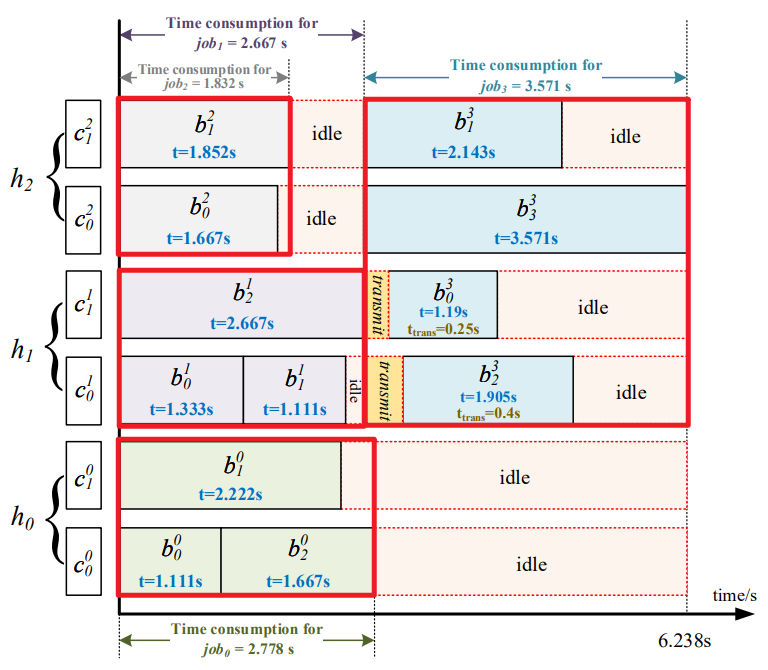
\includegraphics[width=0.9\textwidth]{Fig-CubeLike.png}
			\caption{A simulated image of a solution}
			\label{Fig-Cube}
		\end{center}
	\end{figure}
	
	So the overview of our algorithm is:
	\begin{enumerate}
		\item Regard each job as a cube, generate the initial solution namely initial state in the Simulated Annealing Algorithm. 
		\item Move these cubes and change their width to generate a new state. 
		\item Considering the fixed width of cubes, use Greedy Algorithm to make their length shorter. 
		\item Simulate the calculating process to obtain the final finishing time, namely the energy of the state. 
		\item Perform the annealing, decide whether to accept the new state.
		\item If the temperature and the number of iterations don't reach the standard, go to 2.
		\item Otherwise, end the iteration, the final state is the final solution. 
	\end{enumerate}
 	
 	Here is the pseudo code: \\
 	\begin{algorithm}[H]
 		\KwIn{all the information about hosts, cores, jobs, blocks}
 		\KwOut{the final state}
 		\BlankLine
 		\caption{$schedule()$} \label{Alg-schedule}
 		$init()$\; 
 		$E \leftarrow 0$\; 
 		$tempE \leftarrow 0$\; 
 		$T \leftarrow 1000$\; 
 		$T_e \leftarrow 0.0001$\; 
 		$\beta \leftarrow 0.999$\; 
 		$\delta E \leftarrow 0$\; 
 		$M \leftarrow 100000$\; 
 		\Repeat{$M = 0$}{
 			$move()$\; 
 			$E \leftarrow finishTime()$\; 
 			$tempE \leftarrow temp\_finishTime()$\; 
 			$\delta E \leftarrow tempE- E$\; 
 			\If{$\delta E < 0$}{
 				Accept the new state\; 
 			}
 			\Else{
 				There is a probability of $exp(\frac{-\delta E}{T})$ to accept the new state\; 
 			}
 			$T \leftarrow T*\beta$\; 
 			\If{$T < T_e$}{
 				\textbf{break}\; 
 			}
 			$M \leftarrow M - 1$\;
 		} 
 	\end{algorithm}
	
	\subsection{The Data Structure Mainly Used in the Program} \label{subsec-data}
	We mainly use these data structure in the program: 
	
	\begin{lstlisting}
	vector<int> hostCore;              // The number of cores for each host
	vector<int> jobBlock;              // The number of blocks for each job
	vector<double> Sc;                    // Speed of calculation for each job
	vector<vector<double>> dataSize;      // Job-> block number-> block size
	vector<vector<int>> location;         // Job-> block number-> block location (host number)
	
	vector<double> jobFinishTime;         // The finish time of each job 
	
	vector<vector<tuple<int, int, int>>> runLoc; 
	// 1. Block perspective: job number->block number->(hostID, coreID,rank), rank=1 means that block is the first task running on that core of that host
	
	vector<vector<vector<tuple<int, int, double, double>>>> hostCoreTask; 
	// 2. Core perspective: host->core->task-> <job,block,startRunningTime,endRunningTime>
	
	vector<vector<double>> hostCoreFinishTime; // host->core->finishTime
	
	/* 3. This representation of a solution is used for SAA */
	vector<int>jobCore;  		// The number of cores allocated to each job.
	vector<int>jobOrder;  		//jobOrder[1] stores the first job
	vector<vector<tuple<int, int, vector<int> > > > total_sol;
	//the information of the number of cores are stored in jobCore
	//job-> core ->(hostID, coreID, vector of blockID)
	vector<vector<int> >blockLocation;        
	//job-> blockID-> block destination (hostID)
	
	//modify the solution temporarily
	vector<int>temp_jobCore;
	vector<int>temp_jobOrder;
	vector<vector<tuple<int, int, vector<int> > > >  temp_total_sol;
	vector<vector<int> >temp_blockLocation;
		
	\end{lstlisting}
	
	We will use the third representation of solutions during the annealing. It means different $jobOrder$, $jobCore$ and $total\_sol$ together represent different states. When we generate a new state, we can use it to obtain the finishing time, namely the energy of the state by simulating the calculating process. When we get the final state,  we can transform this representation to the block perspective and core perspective solution. 
	
	\subsection{The Scheme to Generate the Initial State} \label{subsec-initial}
	We already know for one job, if we have decided which cores will be allocated to it, it will be like a cube exsiting on the simulated image of the solution no matter where it is on the image. So we only need to generate the $jobOrder$ and the cores which are allocated to each job. 
	We use random method to generate the two information above. The flow of the scheme is as followed: 
	\begin{enumerate}
		\item Initialize the $jobOrder$ to $1,2,3,..,n$.
		\item For each job, randomly decide the number of cores allocated to it, but restrict that the cores can't more than its blocks.
		\item For each job, randomly decide which cores will be allocated to it. The probability of each core that will be chosen is equal. 
		\item For all the cores allocated to one job, put its blocks into the queues of cores, one for each by order, until the blocks are all put in. 
	\end{enumerate}

	The step $4$ above is meant to make the energy of the initial state higher, to enlarge the effect of moving at the beginning. 
	
	Here is the pseudo code: \\
	\begin{algorithm}[H]
		\KwIn{all the information about hosts, cores, jobs, blocks}
		\KwOut{the initial state}
		\BlankLine
		\caption{$init()$} \label{Alg-init}
		$jobOrder \leftarrow (1, 2, ..., n)$ \;
		\For{i $\leftarrow 0$ to n$- 1$}{
			$jobCore[i] \leftarrow rand()\%min(10,jobBlock[i],m) + 1$ \;
			\For{j $\leftarrow 0$ to jobCore$[i]- 1$}{
				pick a core that hasn't been allocated to $job_i$\;
				$total\_sol[i][j] \leftarrow (host\_id, core\_id, $ process queue for this job$)$\;
			}
			\For{k $\leftarrow 0$ to jobBlock$[i]- 1$}{
				$total\_sol[i][k\%jobCore[i]].queue.push(k)$\;
				$blockLocation[i][k] \leftarrow total\_sol[i][k\%jobCore[i]].host\_id$\;
			}
		}
		$temp\_jobOrder \leftarrow jobOrder$ \;
		$temp\_jobCore \leftarrow jobCore$ \;
		$temp\_total\_sol \leftarrow total\_sol$ \;
		$temp\_blockLocation \leftarrow blockLocation$ \;
	\end{algorithm}
	
	\subsection{The Scheme to Move Blocks to Generate New State} \label{subsec-move}
	The same reason, we only need to change the $job\_order$ and the cores allocated. We have two strategys to change them: 
	\begin{enumerate}
		\item Randomly choose two adjacent jobs, change their order. This will happen at a probability of $P_{co}$. The probability of each job being chosen is equal. 
		\item Randomly choose one job, randomly decide the number of cores allocated to it, but restrict that the cores can't be more than its blocks and ten, then randomly decide which cores will be allocated to it. This will happen at a probability of $P_{rc}$. The probability of each core being chosen is equal. 
	\end{enumerate}

	Here is the pseudo code: \\
	\begin{algorithm}[H]
		\KwIn{the last state}
		\KwOut{the new state}
		\BlankLine
		\caption{$move()$} \label{Alg-move}
		$p \leftarrow rand()\% 2$\;
		\If{n $\geq$ $2$ and p $!= 0$}{                   
			$i \leftarrow rand()\%(n - 1)+1$\;
			$swap(temp\_jobOrder[i], temp\_jobOrder[i + 1])$\;
		}
		$p \leftarrow rand()\% 2$\;
		\If{p $!=0$}{
			$i \leftarrow rand()\% n$\;
			$temp\_jobCore[i] \leftarrow rand()\%min(10,jobBlock[i],m) + 1$ \;
			\For{j $\leftarrow 0$ to temp\_jobCore$[i]- 1$}{
				pick a core that hasn't been allocated to $job_i$\;
				$temp\_total\_sol[i][j] \leftarrow (host\_id, core\_id, $ process queue for this job$)$\;
			}
			$greedy\_allocation(job_i)$\;
		}
		
	\end{algorithm}
	
	\subsection{Make the length of Cubes Shorter by Greedy Algorithm} \label{subsec-GA}
	For one job, when the cores allocated to it have been decided, namely the width of the cube has been fixed, we use Greedy Algorithm to make its length shorter: 
	\begin{enumerate}
		\item Sort all blocks of the job in descending order of data size. 
		\item From the biggest block, compare which core to place it on can minimize the current processing time. Put it on that core. 
		\item Decide all blocks position by 2.
		\item During the process, we can update the $blockLocation$.
	\end{enumerate} 
	
	Here is the pseudo code: \\
	\begin{algorithm}[H]
		\KwIn{$job_i$}
		\KwOut{the schedule scheme for this job}
		\BlankLine
		\caption{$greedy\_allocation(job_i)$} \label{Alg-greedy}
		sort all blocks of $job_i$ in descending order of data size, use $jobBlock\_sorted.push((block\_id, datasize))$\;
		$coreLength \leftarrow (0,0,..,0)$\;
		\For{k $\leftarrow 0$ to jobBlock$[i]$}{
			$b \leftarrow jobBlock\_sorted[k].block\_id$\;
			$min \leftarrow MAX\_LENGTH$\;
			\For{j $\leftarrow 0$ to temp\_jobCore$[i]$}{
				\If{temp\_total\_sol$[i][j]$.host\_id$=$ location$[i][b]$}{
					$ratio \leftarrow 1$
				}
				\Else{
					$ratio \leftarrow 1 + Sc[i]*g(jobCore[i])/St$\; 
				}
				\If{coreLength$[j]+$dataSize$[i][b]*rate<$min}{
					$min \leftarrow coreLength[j] + dataSize[i][k]*ratio$\;
					$index \leftarrow j$\;
				}
			}
			$coreLength[index] \leftarrow min$\;
			$temp\_total\_sol[i][index].queue.push(b)$\;
			$temp\_blockLocaton[i][b] = temp\_total\_sol[i][index].host\_id$\;
		}
	\end{algorithm}
	
	\subsection{The Scheme to Calculate the Energy} \label{subsec-energy}
	We will simulate the calculating process to obtain the final time, namely the energy. The simulating scheme is following: 
	\begin{enumerate}
		\item Initialize a data structure $tf$. It is a two-dimensional array, meaning $host->core->releaseTime$.
		\item According to $jobOrder$ and $total\_sol$, put the cube of each job into the execution queue one by one, like playing $Tetris$.
		\item For every next job, first find the core whose end time is the latest among all the cores allocated to this job and set its end time as the start time of this job.
		\item Then add this job's cube length, namely the total processing time of the job, to the start time, obtain finish time of the job, update $tf$ for all the cores allocated to this job.
		\item Go to 3.
		\item If all the jobs are scheduled, end the cycle. 
	\end{enumerate} 
	
	After simulating, we obtain the final finish time as the energy of the state. 
	
	Here is the pseudo code: \\
	\begin{algorithm}[H]
		\KwIn{$jobOrder$, $jobCore$, $total\_sol$}
		\KwOut{$finishtime$}
		\BlankLine
		\caption{$finishTime()$} \label{Alg-finishtime}
		\For{$i \leftarrow 1$ to $n$}
		{
			$jobi \gets jobOrder[i]$\;
			\For{$j \leftarrow 0$ to $jobCore[jobi] - 1$}
			{
				$host\_id \gets total\_sol[jobi][j].host\_id$\;
				$core\_id \gets total\_sol[jobi][j].core\_id$\;
				$block\_id \gets total\_sol[jobi][j].queue$\;
				$tp_ji \gets 0$\;
				\For{$k = 0$ to $block\_id.size()-1$}
				{
					\If{$location[jobi][block\_id[k]] = blockLocation[jobi][block\_id[k]]$}{
						$tp_ji += dataSize[jobi][block\_id[k]] / (Sc[jobi] \cdot g(jobCore[jobi]))$\;
					}
					\Else{
						$tp_ji += dataSize[jobi][block\_id[k]] / St + dataSize[jobi][block\_id[k]] / (Sc[jobi] \cdot g(jobCore[jobi]))$\;
					}
				}
				$tp_i[j] \gets tp_ji$\;
				\If{$t_i < tf[host\_id][core\_id]$}{
					$t_i \gets tf[host\_id][core\_id]$\;
				}
			}
			$tf\_jobi \gets t_i + max(tp_i[])$\;
			update $tf[host\_id][core\_id]$ for all cores allocated to $jobi$\;
			\If{$finishtime < tf\_jobi$}{
				$finishtime \gets tf\_jobi$\;
			} 
			%find max tf[][] for every core
		}
		\Return{$finishtime$}\;
	\end{algorithm}
	
	\section{Results and Parameter Experiments} \label{sec-experiment}
	\subsection{Final Results} \label{subsec-res}
	We first give a sample result of our algorithm: 
	
	For $Task 1$: 
	\begin{figure}[H]
		\begin{center}
			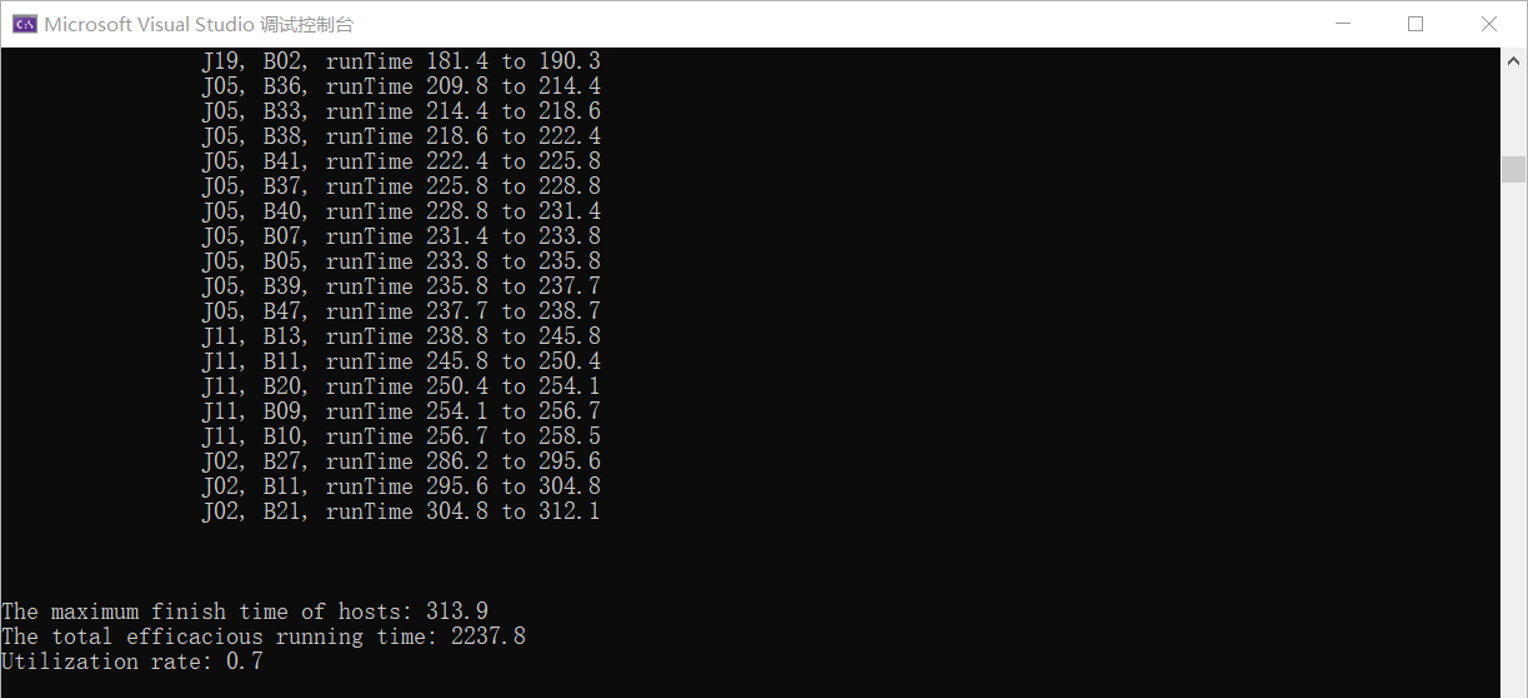
\includegraphics[width=0.9\textwidth]{Fig-task1-res-new.png}
			\caption{The sample result of Task1}
			\label{Fig-task1-res}
		\end{center}
	\end{figure}
	
	For $Task 2$: 
	\begin{figure}[H]
		\begin{center}
			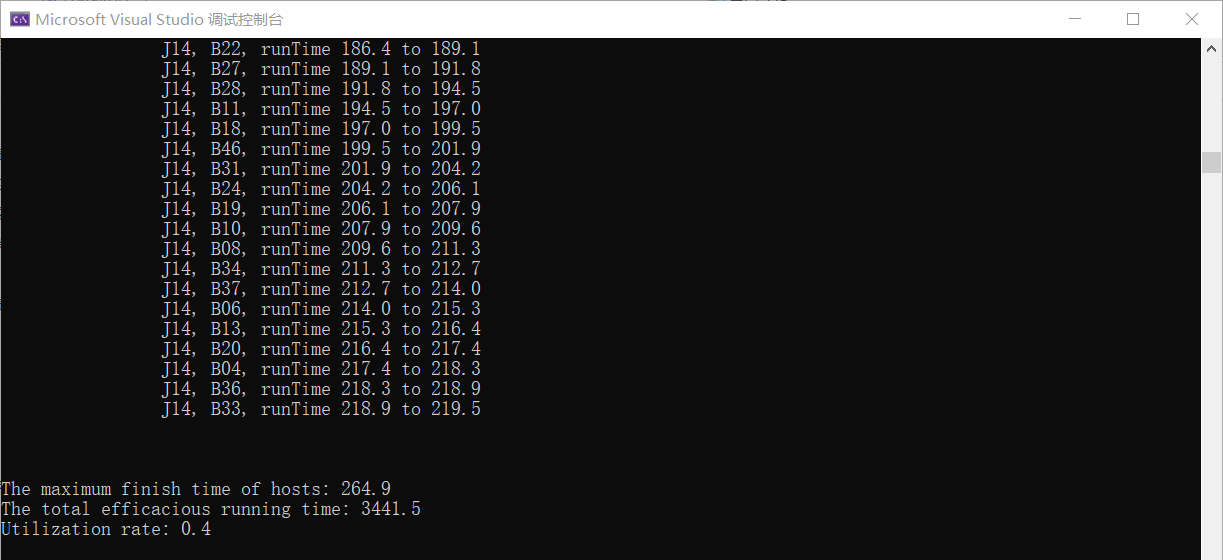
\includegraphics[width=0.9\textwidth]{Fig-task2-res.png}
			\caption{The sample result of Task2}
			\label{Fig-task2-res}
		\end{center}
	\end{figure}
	
	The complete output can be checked in \texttt{task1\_case1\_01.txt} and \texttt{task2\_case1\_01.txt}. 
	
	We can visualize the annealing process: 
	
	For $Task 1$: 
	\begin{figure}[H]
		\begin{center}
			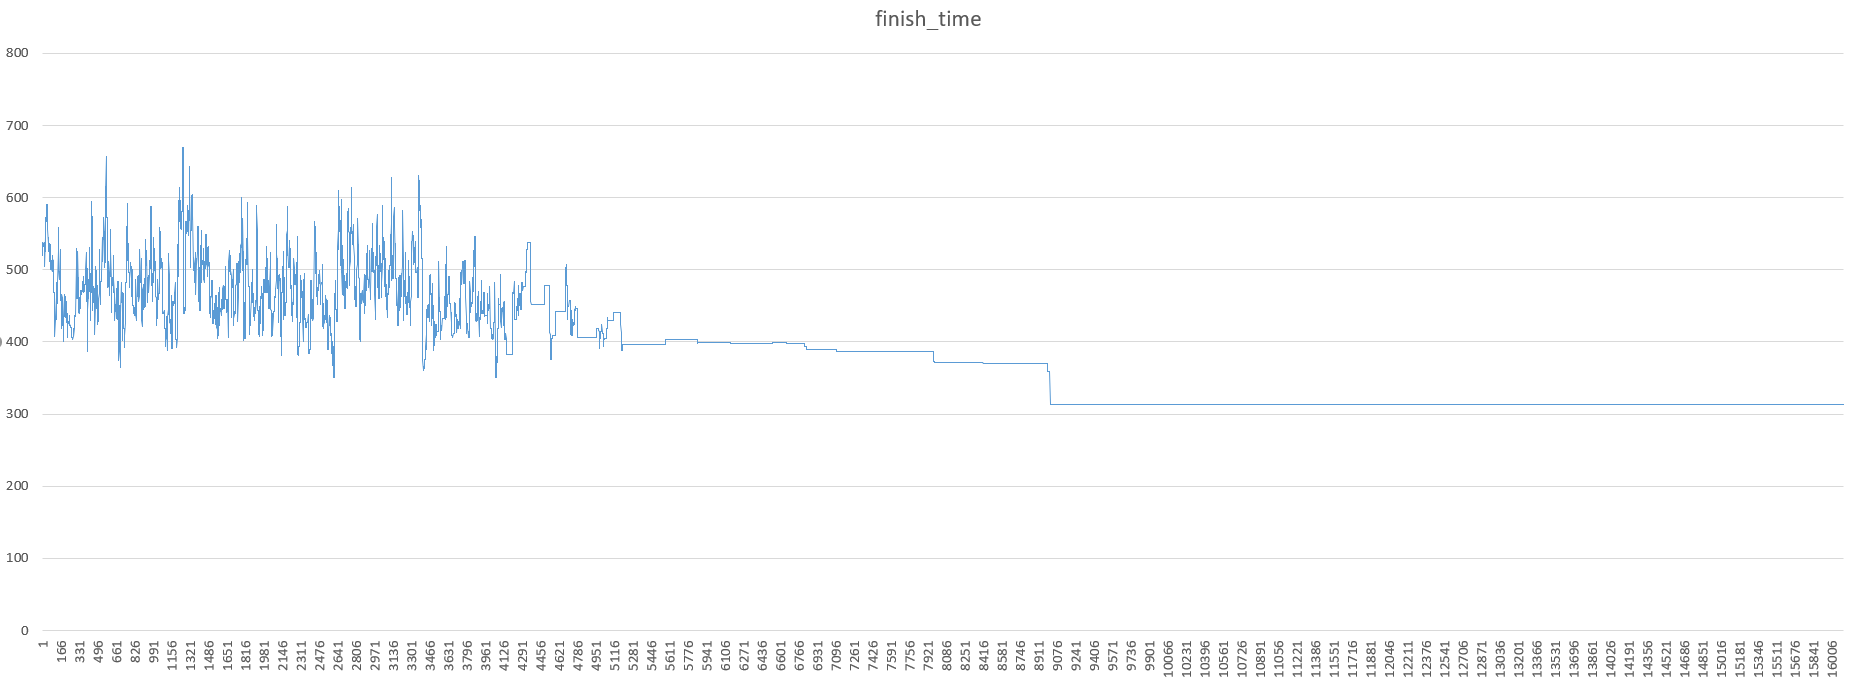
\includegraphics[width=0.9\textwidth]{Fig-task1-annealing.png}
			\caption{The annealing process of Task1}
			\label{Fig-task1-annealing}
		\end{center}
	\end{figure}

	For $Task 2$: 
	\begin{figure}[H]
		\begin{center}
			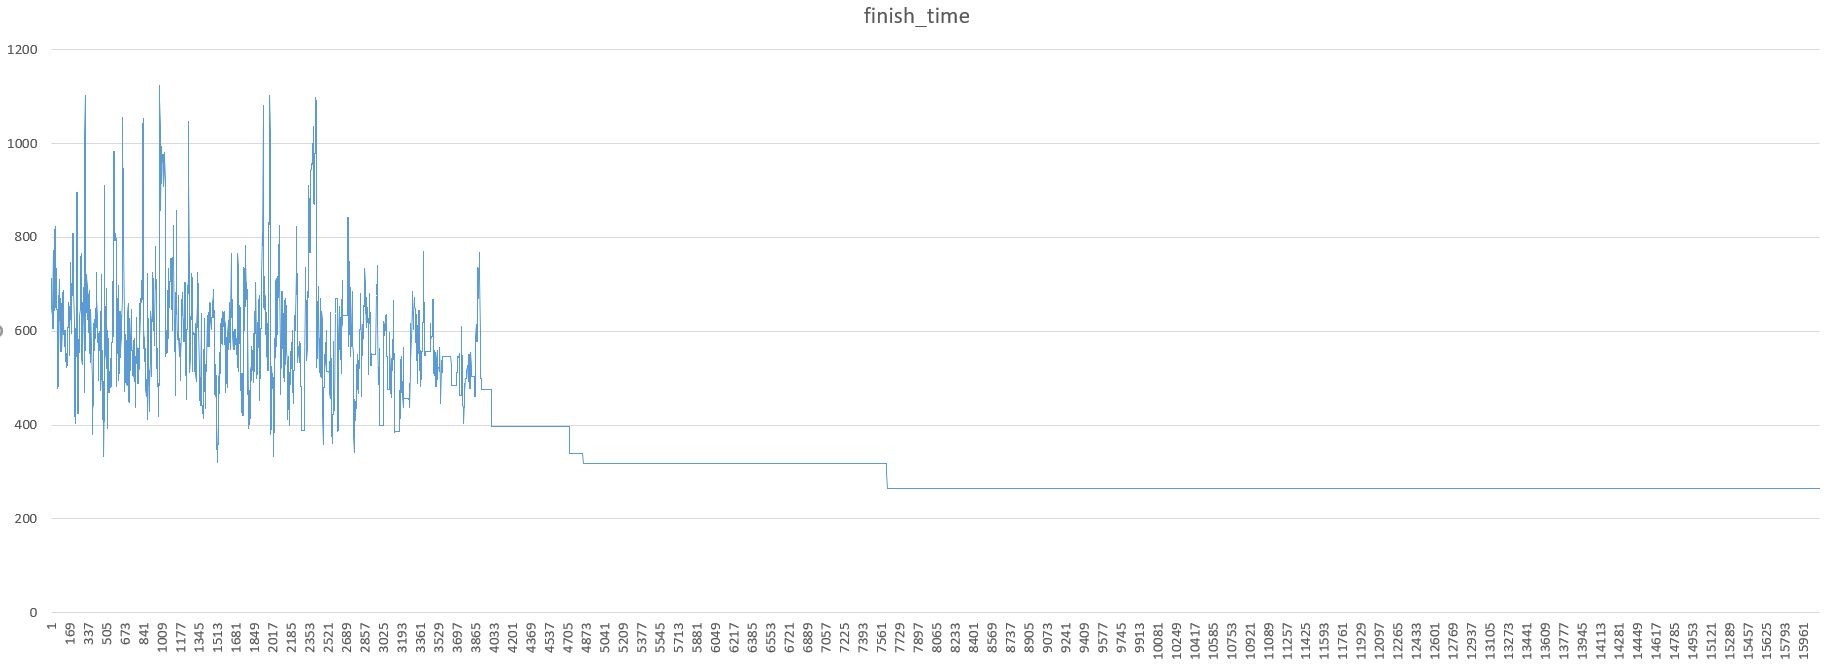
\includegraphics[width=0.9\textwidth]{Fig-task2-annealing.png}
			\caption{The annealing process of Task2}
			\label{Fig-task2-annealing}
		\end{center}
	\end{figure}
	
	\subsection{Parameter Experiments} \label{subsec-expr}
	In this section, we will use different parameters to test the simulated annealing algorithm and compare the different results. 
	
	For $Task1$:
	
	\begin{table}[H]
		\caption{The average result of Task1 for different parameters}
		\begin{center}
			\resizebox{0.8\textwidth}{!}{
			\begin{tabular}{c|ccc}
				\hline
				& $P_{co}=0.25$ & $P_{co}=0.5$ & $P_{co}=0.75$ \\ \hline
				$P_{rc}=0.25$ & 361.10    & 356.70   & 353.16   \\
				$P_{rc}=0.5$ & 360.54   & 358.16  & 349.98   \\
				$P_{rc}=0.75$ & \cellcolor[HTML]{FFFFC7}344.74   & 354.98  & 354.90    \\ \hline
			\end{tabular}}
			\label{table-task1}
		\end{center}
	\end{table}

	For $Task2$:
	
	\begin{table}[H]
		\caption{The average result of Task2 for different parameters}
		\begin{center}
			\resizebox{0.8\textwidth}{!}{
				\begin{tabular}{c|ccc}
					\hline
					& $P_{co}=0.25$ & $P_{co}=0.5$ & $P_{co}=0.75$ \\ \hline
					$P_{rc}=0.25$ & 352.64    & 350.56   & 354.18   \\
					$P_{rc}=0.5$ & 332.76   & \cellcolor[HTML]{FFFFC7}315.92  & 331.48   \\
					$P_{rc}=0.75$ & 316.10   & 324.28  & 323.02    \\ \hline
			\end{tabular}}
			\label{table-task2}
		\end{center}
	\end{table}
	
	However, the parameters will be affected by the test case itself. The results we get may not be universal. 
	
	
	\section{Algorithm Analysis} \label{sec-analysis}
	In this section, we will analyze the time complexity of our algorithm. And we will justify whether this problem is NP-complete.
	\subsection{Time Complexity} \label{subsec-time}
	\begin{enumerate}
		\item The times of annealing is 
		\[
			min(M, log_\beta \frac{T_e}{T_0})
		\]
		\item In $move()$, the time complexity of changing order is $O(1)$. As for choosing cores, the max number of cores allocated to one job is $10$. Assume that we need $X$ times to pick out $10$ different cores for one job, $X_i$ is how many times it needs to pick a new core when it has already picked $i-1$ cores. $X_i$ follows the a geometric distribution. 
		\[E(X_i) = \frac{1}{p_i} = \frac{m}{m-i+1}
		\]
		$p_i$ means the probability of choosing a new core when it has already picked $i-1$ cores. \\
		Because $X = \sum_{i = 1}^{10} X_i$, 
		\[E(X) = \sum_{i = 1}^{10} \frac{m}{m-i+1} \rightarrow 10
		\]
		\item The time complexity of $greedy\_allocation(job_i)$ is $O(jobBlock[i]\cdot jobCore[i])$. Because $jobCore[i] \leq jobBlock[i]$, the time complexity is actually $O(jobBlock[i]^2)$. Therefore, the time complexity of $move()$ is $O(10 \cdot max(jobBlock[])^2) \sim O(max(jobBlock[])^2)$. 
		\item $finishTime()$ essentially iterates through all the blocks and then finds the max finish time on cores. So the time complexity is $O(\sum_{i = 0}^{n-1} jobBlock[i] + m)$. 
		\item The other functions just have the same time complexity of the functions above or smaller.
	\end{enumerate}
	So the time complexity of the whole algorithm is
	\[O(min(M, log_\beta \frac{T_e}{T_0})\cdot [max(jobBlock[])^2 + \sum_{i = 0}^{n-1} jobBlock[i] + m])
	\]

	\subsection{Explanation to Greedy Thoughts} \label{subsec-exptogreedy}
	First of all, we would like to explain how we figure out the greedy algorithm used for shortening the length of cubes of jobs. 
	
	We do the following qualitative analysis:
	\begin{enumerate}
		\item The length of a job's cube must be larger than the max size of its blocks.
		\item Every time we put a new block into the cores' queue, the increase of the length is not bigger than the size of this block. 
		\item We want the idle part to be as small as possible. And the max idle part is the gap between the shortest queue and the longest queue.
		\item If adding a block makes the longest queue changes, we want the increase of the length of the cube is the smallest.  
	\end{enumerate}

	Based on them, we designed the $greedy\_allocation()$. It obtain a good enough soltion for each job in the simplfied version. Because the processing time for each block is proportional to its size. But it isn't optimal. We will explain it in Section~\ref{subsec-npc}. 
	
	In the comprehensive version, the transmission time will affect the actual processing time of a job. Because some blocks have no need to transmit, while the others need. The actual processing time is still proportional to its size, but the ratio is different for each block. So the Greedy Algorithm can't work better than it does in the simplified version. However, because the transmission time of each job is one tenth of the processing time or less, the greedy algorithm can still give a good solution. 
	
	\subsection{NP-complete Proof} \label{subsec-npc}
	\subsubsection{NP}
	If we know the minimum finish time and the list of places of all blocks, we use function $finishtime()$ to certificate, which leads to the polynomial time complexity.
	
	\subsubsection{Partition Problem}
	The partition problem, or number partitioning, is the task of deciding whether a given multiset $S$ of positive integers can be partitioned into two subsets $S_1$ and $S_2$ such that the sum of the numbers in $S_1$ equals the sum of the numbers in $S_2$. The partition problem is NP-complete\cite{ref_article1}.
	
	\subsubsection{NP-complete of Simplest Case}
	We consider the simplest case that there is only one job allocated onto $2$ cores. 
	
	Consider the partition problem about the set of blocks' working time $A$. If we find a solution of the problem that there is no idle time ($finishtime = \frac{1}{2}\sum_{a \in A}a$), we get a solution of partition problem about $A$, and if there is idle time existing ($finishtime \neq \frac{1}{2}\sum_{a \in A}a$), we know that there is no solution of this partition problem.
	
	The reduction takes $O(n)$ time complexity to sum all elements in $A$ and $O(1)$ time of the "black box" algorithm, so it is a polynomial reduction, which means the simplest case is NP-complete.
	
	\subsubsection{NP-complete of General Case}
	It is obvious that the general case, with more jobs and more blocks, is harder than the simplest case. The discussion below is based on the assumption that we have an algorithm $f(m, n)$ to solve $m$ job case on $n$ cores, where $m$ and $n$ are arbitrary. Single-host or multi-host doesn't matter, because we only need to add a special parameter on the size of blocks.
	
	Considering the simplest case, we can set $m = 1$ and $n = 2$, then $f(1, 2)$ is an algorithm to solve it, which leads to a polynomial reduction. Since the simplest case is NP-complete, the general case is NP-complete as well.
	
	
	\subsection{Experiment on Greedy Quality}
	In Section~\ref{subsec-npc}, we prove that minimizing the length of one job cube with fixed core number is an NP-complete problem. If $P\neq NP$, we can't find a optimal solution in polynomial time. The greedy algorithm we used for the simplified version is not optimal. (For the comprehensive version it is obviously not the optimal.) Therefore, in the simplified version, we compare the solution which our greedy algorithm gives to the theoretical optimal solution, in order to test whether it gives a good enough solution. 
	The theoretical optimal cube length for $job_i$ is 
	$$
	\frac{\sum_{k = 0}^{jobBlock[i]-1} datasize[i][k]}{jobCore[i]}
	$$
	It is easy to know that the actual optimal cube length must not be shorter than the theoretical one. 
	
	\begin{figure}[H]
		\begin{center}
			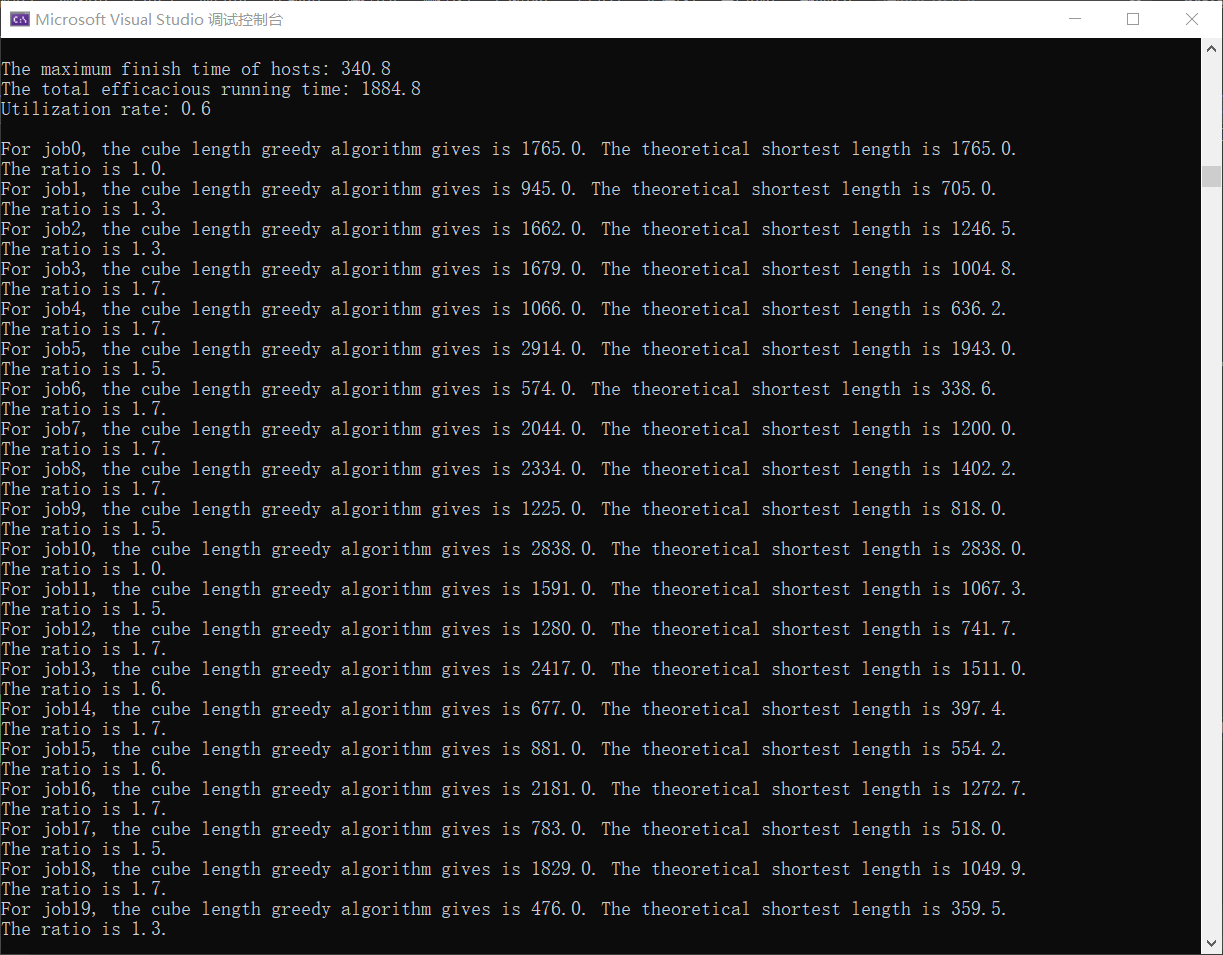
\includegraphics[width=0.9\textwidth]{Fig-task1-testforgreedy.png}
			\caption{Comparation between greedy solution and theoretical optimal solution}
			\label{Fig-task1-testforgreedy}
		\end{center}
	\end{figure}

	The complete output can be checked in \texttt{task1\_case1\_01 (2).txt}. 
	
	We can see the cube length greedy algorithm gives is not more than $2$ times the theoretical optimal one. For the actual optimal solution this ratio may be smaller. And sometimes it gives a result as good as the theoretical optimal one. Therefore, we think our greedy algorithm gives a good enough solution. 
	 
	
	\section{Experimemt Based on A Completely Random Move} \label{random}
	In Section~\ref{sec-analysis}, we explain and test the quality of the greedy algorithm we used. And we can know for multiple host version greedy algorithm is not optimal. So we design another move method which not only moves the job cubes, but also moves the blocks in each job cube. Namely, we will use a completely random strategy to generate new states and check if it can give us a better result. 
	The new move strategy is following:
	\begin{enumerate}
		\item Randomly choose two adjacent jobs, change their order. This will happen at a probability of $P_{co}$. The probability of each job that will be chosen is equal. 
		\item Randomly choose one job, randomly choose a core that has been allocated to it, change it to another core that hasn't been allocated to it. This will happen at a probability of $P_{rc}$. The probability of each core that will be chosen is equal. 
		\item Randomly choose one job $job_i$, randomly choose a core $core_j$ that has been allocated to $job_i$, randomly choose a block $B_k$ that on this core. Then randomly generate a core index. The core index will be in the range of $[0, temp\_jobCore[i]]$, but it can't be the $core_j$. This will happen at a probability of $P_{mb}$. 
		
		\par If the core index is equal to $temp\_jobCore[i]$, it means we will give a new core to $job_i$. We randomly choose this new core from the cores which haven't been allocated to $job_i$. If there is only one block on $core_j$, we will directly change $core_j$ to this new core. If there are more than one block on $core_j$, we add this new core to $job_i$ and move $B_k$ from $core_j$ to this new core. 
		\par If the core index is smaller than $temp\_jobCore[i]$, it means we will move $B_k$ from $core_j$ to another core of $job_i$. If there is only on block on $core_j$, we will delete $core_j$ from $job_i$ after moving. 
	\end{enumerate}

	However, in experiment, though we amplify the probability of each move stategy and the iteration times, we can't get a better result than that the greedy algorithm gives. 
	
	\begin{figure}[H]
		\begin{center}
			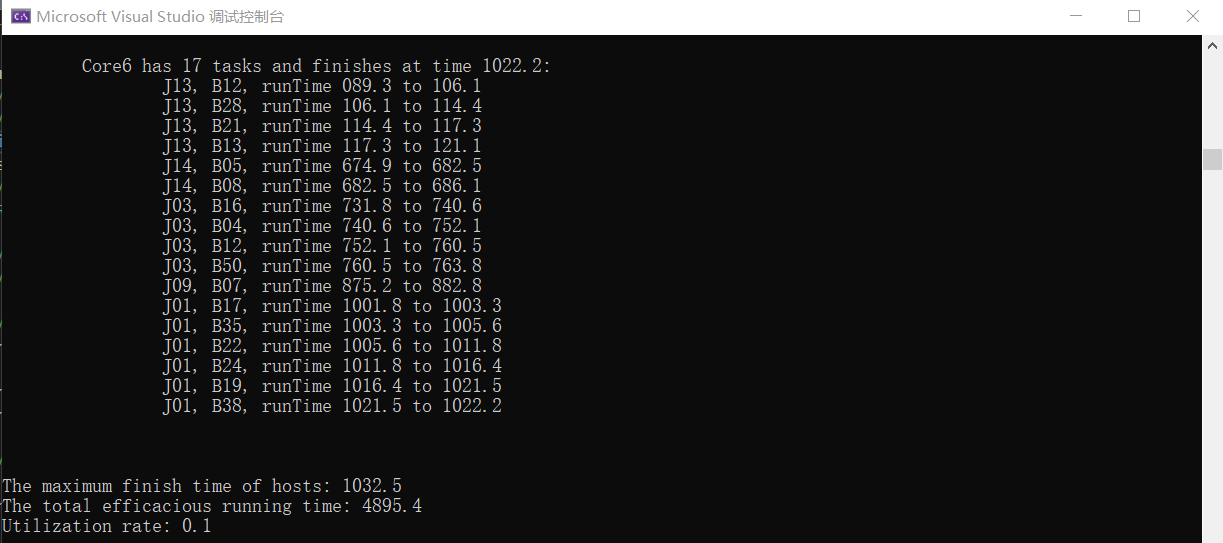
\includegraphics[width=0.9\textwidth]{Fig-task2-res-random.png}
			\caption{The result of Task2 given by completely random move strategy}
			\label{Fig-task2-res-random}
		\end{center}
	\end{figure}
	
	This is because each movement of this strategy is too small. If we change the Simulated Annealing Algorithm, let it only accepts the state with lower energy, the result will be improved a little. But it is still much worse than the greedy. 
	
	\begin{figure}[H]
	 	\begin{center}
	 		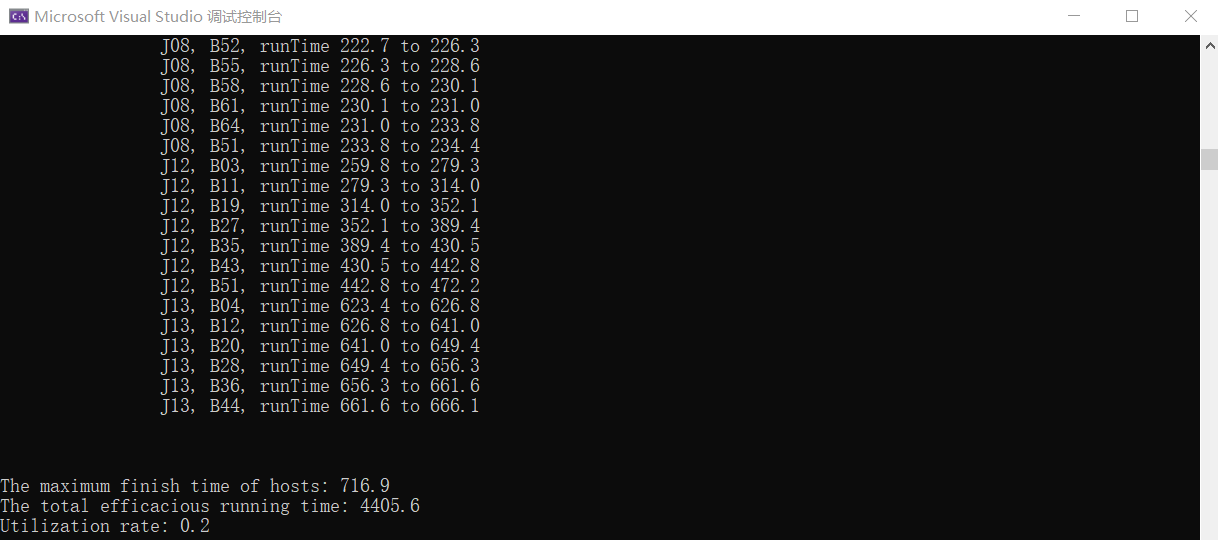
\includegraphics[width=0.9\textwidth]{Fig-task2-res-random-imp.png}
	 		\caption{The result of Task2 given by completely random move strategy if SAA only accepts states with lower energy}
	 		\label{Fig-task2-res-random-imp}
	 	\end{center}
	\end{figure}

	If we apply this changed SAA on the greedy version, sometimes it can give a better solution than the average result of the original SAA. But it can hardly give a solution better than the best result the original SAA ever gives. The reason is that it may cause the state to stay at the locally optimal solution. When the solution is good enough, it is hard for the changed SAA to move anymore. 
	
	\section{Summary}
	In this article, we focus on designing an algorithm for solving resource scheduling problems in Hadoop. The algorithm we design is based on simulated annealing algorithm and greedy algorithm to give an approximate solution to the problems of both simplified and comprehensive versions. We also do some experiments on parameters in the algorithm but the results we get are for the special test cases and not universal. During analyzing the complexity and other quality of our algorithm, we found that the problem is NP-complete. Though we hope our greedy algorithm is optimal for one job in the simplified version, it is an NP-complete problem, we can’t find its optimal solution in polynomial time. So we compare the greedy solution to the theoretical optimal solution to prove the greedy one is good enough. Finally, we use a completely random move strategy to try to find a better solution for the comprehensive version. But the result is that it can’t work better than the greedy. 
	
	In general, the SACG is our feasible but imperfect answer to resource scheduling problem in Hadoop.
	
	\section*{Acknowledgements}
	This problem is motivated from a real-world cloud service corporation. It is formulated by Prof. Xiaofeng Gao (gao-xf@cs.sjtu.edu.cn) from Department of Computer Science and Engineering at Shanghai Jiao Tong University. Yue Ma scribed and modified the project. Yangyang Bao provided the example in Task 1. Zhen Sun provided the example in Task 2. Wanghua Shi provided the test data and source code. Jiale Zhang, Tianyao Shi helped on proofreading and provided many suggestions.
	
	% Here is your acknowledgements. You may also include your feelings, suggestion, and comments in the acknowledgement section.
	Thank assistants Fang Hongjie, Lv Jialin and Shi Wanghua. They gave so many instructive suggestions to our group.
	
	Thank professor Gao Xiaofeng. The problem she assigned helps us understand the actual case in real world better and improves our abilities. 
	
	Every group member has learned a lot from this project. 
	
	\textbf{Zhenran Xiao:} Figuring out this problem is more and more interesting during the whole process. At the beginning, I just feel anxious and nervous. I was worried whether we can give a result. But as the project progressed, I had fun, especially when I drew the picture of the annealing process. I feel the charm of the Simulated Annealing Algorithm. 
	
	When I gave out the greedy algorithm used for one job on single host(I need to state I think out this by myself instead of searching it out on the Internet), I actually don't know how to prove whether it is optimal. Finally, we found out that the problem is an NP-complete problem. We can't find a optimal solution in polynomial time. 
	
	Really thankful to my groupmates, they did much difficult work in the project and answered many questions I asked. Trying to express everyone's awesome ideas clearly in the article is a challenge as well. I really learned a lot.
	
	\textbf{Zichun Ye:} As a member of the group, my job is implementing the main part of the code, debugging and providing the test answer. During this process, I faced many difficulties including setting the variables, finding errors through hundreds of lines and reading others’ code. I took notes of all these variables to make coding easier. In the end, the program runs smoothly without annoying bugs. 
	
	I learned that before writing the code, I shall have clearheaded logic, otherwise it’s destructive to modify the code. Writing notes in the code is also essential because your teammates also need to understand what you write. 
	
	Thank Xiao Zhenran and Long Mabiao. They supported me a lot and did an excellent job in this project.
	
	\textbf{Mabiao Long:} Since we haven’t learned about the NP problem at first, we learned from other similar problems on the Internet and finally chose the SA algorithm, instead of dynamic programming, to deal with the case that a large amount of data may appear. I believe that learning from others will be a shortcut while facing engineering problems, though it may be a hard problem or even an unsolvable problem now, there may be some tips or thoughts that lead to the correct way. 
	
	I worked on two functions, $finishtime()$ and $write\_back()$. Based on a concise and effective data structure, it is easier to work out. I also worked on the proof of NP-complete, which deepened my understanding of computational complexity and taught me that some seemingly simple questions can be difficult.
	
	Thanks for my teammates, Zhenran Xiao and Zichun Ye, they inspired me and corrected my mistakes, which taught me a lot during these weeks.
	
	
	%
	% ---- Bibliography ----
	%
	% BibTeX users should specify bibliography style 'splncs04'.
	% References will then be sorted and formatted in the correct style.
	%
	\newpage
	\bibliographystyle{splncs04}
	%\bibliography{refpaper.bib}
	\begin{thebibliography}{8}
		\bibitem{ref_url1}
		shiwanghua/SharedFiles, \url{https://github.com/shiwanghua/SharedFiles/tree/Project-CodeDemo}. Last accessed 15 May 2022
		
		\bibitem{ref_url2}
		yunzhe99/Hadoop\_Scheduling, \url{https://github.com/yunzhe99/Hadoop_Scheduling}. Last accessed 11 Dec 2021
		
		\bibitem{ref_url3}
		模拟退火(simulated annealing)算法详解, \url{https://blog.csdn.net/weixin_60737527/article/details/123936955?utm_medium=distribute.pc_relevant.none-task-blog-2~default~baidujs_baidulandingword~default-0.pc_relevant_default&spm=1001.2101.3001.4242.1&utm_relevant_index=3}. Last accessed 3 Apr 2022
		
		\bibitem{ref_article1}
		Hayes, Brian (March–April 2002), "The Easiest Hard Problem" (PDF), American Scientist, Sigma Xi, The Scientific Research Society, vol. 90, no. 2, pp. 113–117, JSTOR 27857621
		
	\end{thebibliography}
	
	\newpage
	\begin{appendices}
		\section*{Appendix A}
		\begin{table}[H]
			\caption{Symbols and Definitions}
			\begin{center}
				\begin{tabular}{c|c}
					\toprule
					\textbf{Symbols} &\textbf{Definitions}  \\
					\midrule
					$n$ & The number of jobs  \\ 
					$m$ & The number of cores \\
					$q$ & The number of hosts  \\ 
					$job_i$, $J$ & $job_i$ is the $i$-th job. The job set is $J=\{job_0, \cdots, job_{n-1}\}$. \\ 
					$h_l$, $H$ & $h_l$ is the $l$-th  host. The host set is $H=\{h_0, \cdots, h_{q-1}\}$. \\ 
					$m_l$ & The number of cores on host $h_l$\\
					$c^l_j$, $C_l$ & $c^l_j$ is the $j$-th core on host $h_l$. $C_l$ is the set of cores on host $h_l$.\\ 
					$C$ & The set of cores. $C=\{c_0,\cdots,c_{m-1}\}$ for single-host. $C=\cup_{l=0}^{q-1} C_l$ for multi-host.\\
					$b^i_k$& The block of $job_i$ whose id is $k$\\
					$B^i_{j}$ & The set of data blocks of $job_i$ allocated to core $c_j$ \\
					$B^i$ & The set of data blocks of $job_i$ \\ 
					$B^i_{lj}$ & The set of data blocks of $job_i$ allocated to core $c^l_j$ \\
					$\widetilde{B}^i_{lj}$ & The set of data blocks of $job_i$ allocated to core $c^l_j$ but not initially stored on $h_l$\\
					$size(\cdot)$ & The size function of data block\\
					$g(\cdot)$ &  The computing decaying coefficient caused by multi-core effect\\
					$s_i$ & The computing speed of $job_i$ by a single core\\
					$s_t$ & The transmission speed of data \\
					$e_i$ & The number of cores processing $job_i$\\ 
					$t_i$ & The time to start processing $job_i$\\
					$tp^i_j$, $tf^i_{j}$ & The processing time / finishing time of core $c_j$ for $job_i$\\
					$tp^i_{lj}$, $tf^i_{lj}$ & The processing time / finishing time of core $c^l_j$ for $job_i$\\
					$tf(job_i)$ & The finishing time of $job_i$ \\
					$state_i$ & The $i$th state of the material or solution \\
					$E(i)$ & The energy of $state_i$ \\
					$K$ & Boltzmann's constant \\
					$T$ & The temperature of current state \\
					$T_i$ & The temperature of $state_i$ \\
					$T_e$ & The final temperature \\
					$\beta$ & The rate of temperature fall \\
					$M$ & The maximum number of iterations \\
					$\delta E$ & The change of energy between two states \\
					$P_{co}$ & The probability changing two job's order \\
					$P_{rc}$ & The probability re-choosing cores for one job \\
					$X$ & Times to pick out $10$ different cores for one job \\
					$X_i$ & Times it needs to pick a new core when it has already picked $i-1$ cores \\
					$p_i$ & The probability of choosing a new core when it has already picked $i-1$ cores \\
					$P_{mb}$ & The probability move blocks for one job \\
					%  & \\
					%  & \\
					%  & \\
					%  & \\
					%  & \\
					%  & \\ 
					
					\bottomrule
					%\multicolumn{4}{l}{$^{\mathrm{a}}$Sample of a Table footnote.}
				\end{tabular}
				\label{tabSYMBOLS}
			\end{center}
		\end{table}
		
		\section*{Appendix B}
		\begin{figure}[H]
			\begin{center}
				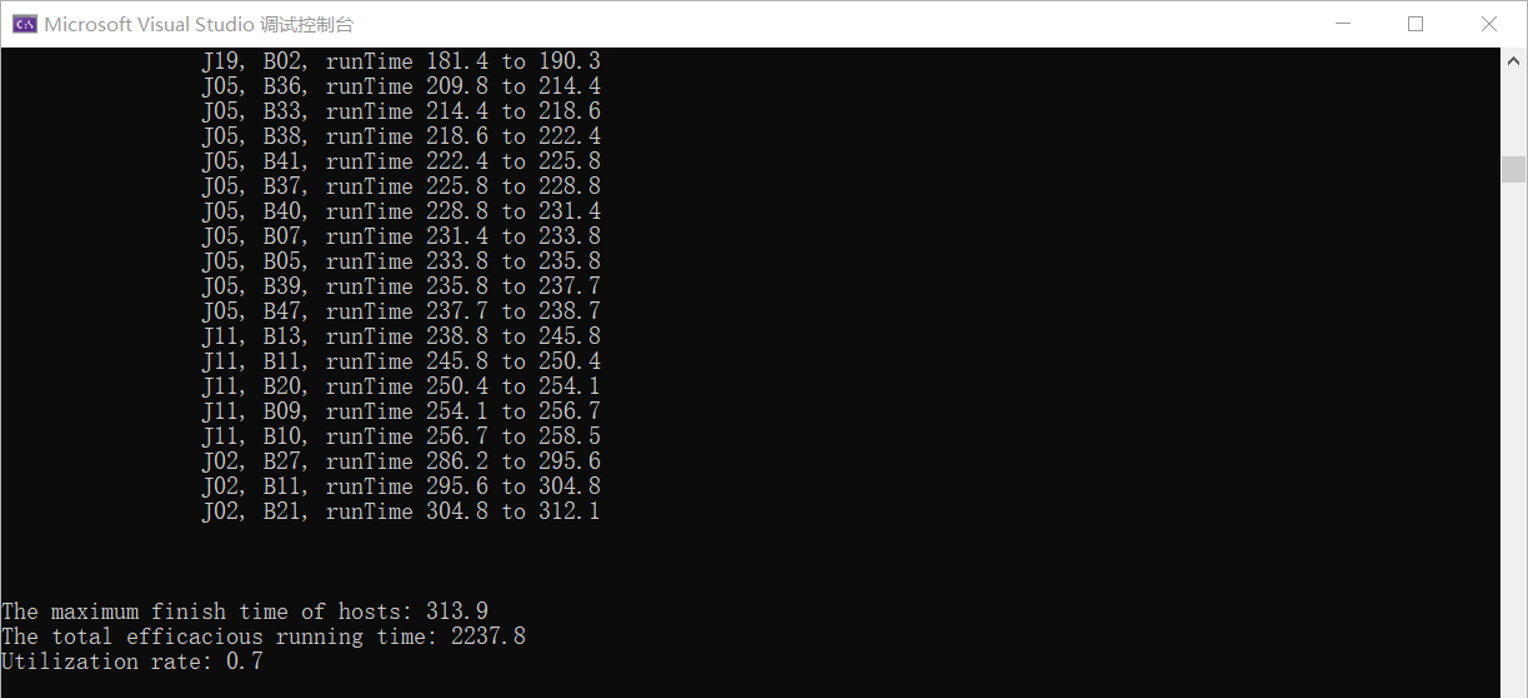
\includegraphics[width=0.9\textwidth]{Fig-task1-res-new.png}
				\caption{The best result of Task1 we have ever gotten}
				\label{Fig-task1-best}
			\end{center}
		\end{figure}
		The complete output can be checked in \texttt{task1\_case1\_01.txt}. 
	
		\begin{figure}[H]
			\begin{center}
				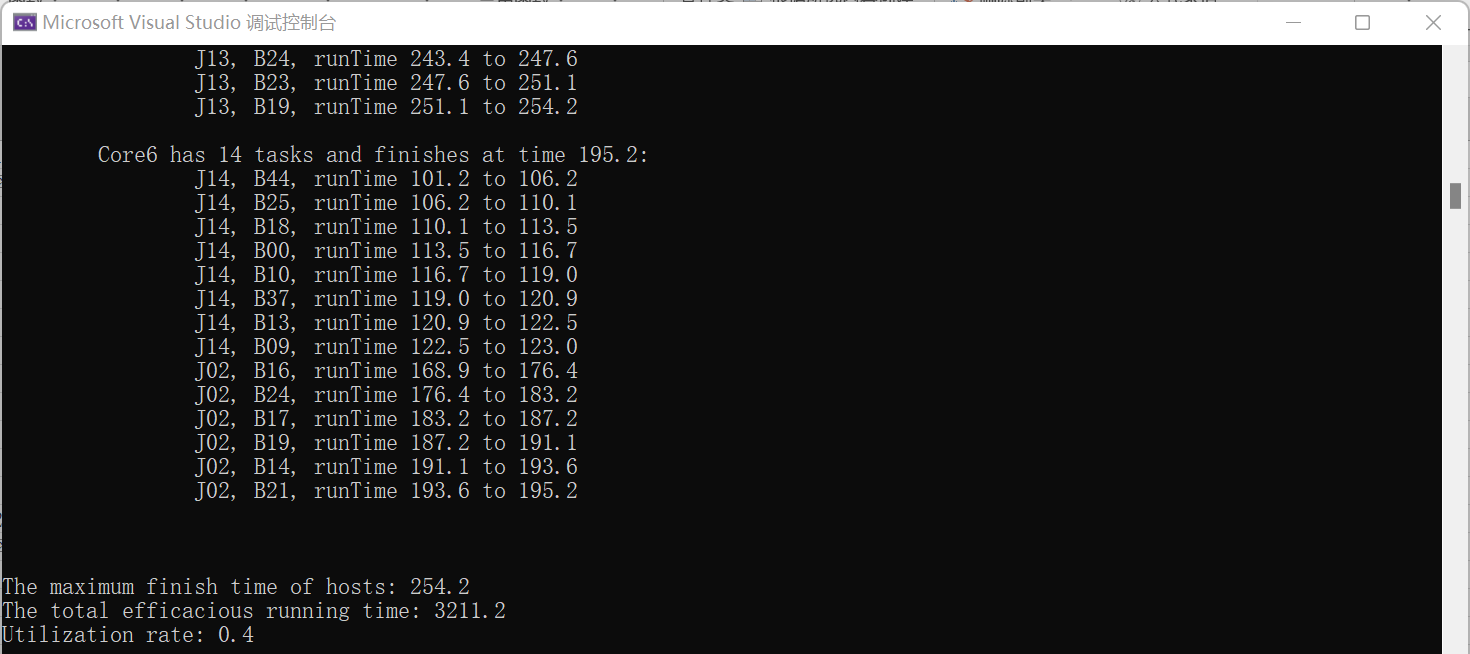
\includegraphics[width=0.9\textwidth]{Fig-task2-res-new.png}
				\caption{The best result of Task2 we have ever gotten}
				\label{Fig-task2-res-new}
			\end{center}
		\end{figure}
		The complete output can be checked in \texttt{task2\_case1\_01 (2).txt}. 
		
	\end{appendices}
	
	%\begin{comment}
	%\begin{thebibliography}{8}
		
	%\bibitem{ref_article}
	%Author, F.: Article title. Journal \textbf{2}(5), 99--110 (2016)
	% \bibitem{dean2008mapreduce}
	% Dean J, Ghemawat S. MapReduce: simplified data processing on large clusters[J]. Communications of the ACM, 2008, 51(1): 107-113.
	
	% \bibitem{ref_lncs1}
	% Author, F., Author, S.: Title of a proceedings paper. In: Editor,
	% F., Editor, S. (eds.) CONFERENCE 2016, LNCS, vol. 9999, pp. 1--13.
	% Springer, Heidelberg (2016).
	
	% \bibitem{ref_book1}
	% Author, F., Author, S., Author, T.: Book title. 2nd edn. Publisher,
	% Location (1999)
	
	% \bibitem{ref_proc1}
	% Author, A.-B.: Contribution title. In: 9th International Proceedings
	% on Proceedings, pp. 1--2. Publisher, Location (2010)
	
	% \bibitem{ref_url1}
	% LNCS Homepage, \url{http://www.springer.com/lncs}. Last accessed 4
	% Oct 2017
	 
	%\end{thebibliography}
	%\end{comment}

	
\end{document}


